\documentclass{article}

\usepackage{fullpage}
\usepackage{url}
\usepackage{graphicx}
\usepackage{amsmath}
\usepackage{physics}
\usepackage{mathtools}

\DeclareMathOperator{\erfi}{erfi}
\newcommand{\R}{\ensuremath{\mathbb{R}}}

\title{Quantum Mechanics I Excercise 3}
\author{Idan Stark}
\date{\today}

\begin{document}
\maketitle

\section{The semiclassical limit for momentum space path integral}
Following the same method as in the notes, we start from the path integrals in phase space formulation:
\begin{equation}
    K(x_f, t_f : x_i, t_i) = \int Dx(t) Dp(t) \exp[\frac{i}{\hbar}S\left[p(t), x(t)\right]]
\end{equation}
With the action
\begin{equation}
    S\left[p(t), x(t)\right] = \int_{t_i}^{t_f} dt \left[p(t) \frac{dx(t)}{dt} - H(p(t), x(t))\right]
\end{equation}
Since we want this in the momentum space:
\begin{equation}
\begin{gathered}
    K(p_f, t_f : p_i, t_i) = \bra{p_f}U(t_f, t_i)\ket{p_i} =
    \int dx_i dx_f \bra{p_f}\ket{x_f}\bra{x_f}U(t_f, t_i)\ket{x_i}\bra{x_i}\ket{p_i} =
    \\
    = \frac{1}{2\pi\hbar}\int dx_i dx_f e^{-ip_fx_f/\hbar}K(x_f, t_f : x_i, t_i)e^{ip_ix_i\hbar} =
    \\
    = \frac{1}{2\pi\hbar}\int dx_i dx_f e^{\frac{i}{\hbar}(p_ix_i - p_fx_f)}K(x_f, t_f : x_i, t_i)
\end{gathered}
\end{equation}
Integrating by parts the $p\dot{x}$ in the action, we can see that the full exponent is:
\begin{equation}
\begin{gathered}
    \tilde{S}\left[p(t), x(t)\right] = S\left[p(t), x(t)\right] + p_ix_i - p_fx_f =
    \\
    = \int_{t_i}^{t_f} dt \left[p(t) \frac{dx(t)}{dt} - H(p(t), x(t))\right] + p_ix_i - p_fx_f = 
    \\
    = \int_{t_i}^{t_f} dt \left[-x(t) \frac{dp(t)}{dt} - H(p(t), x(t))\right]
\end{gathered}
\end{equation}
In the limit $\hbar \rightarrow 0$, the stationary solutions will dominate the integral:
\begin{equation}
    \delta \tilde{S} = 0
\end{equation}
We can see here the classical legendere transform over the Hamiltonian that gives the Lagrangian. We can find the EOM using the E-L equation for both $p$ and $x$. The EOMs that stem from this action are the canonical relations:
\begin{equation}
    \frac{dx_{cl}(t)}{dt} = \left.\frac{\partial H(p(t),x(t))}{\partial p(t)}\right|_{p=p_{cl}, x=x_{cl}}
    \qquad
    \frac{dp_{cl}(t)}{dt} = -\left.\frac{\partial H(p(t),x(t))}{\partial x(t)}\right|_{p=p_{cl}, x=x_{cl}}
\end{equation} 
Finally, since the path is between predetermined momentum states, they will now give the boundary conditions:
\begin{equation}
\begin{gathered}
    p_{cl}(t_i) = p_i \qquad p_{cl}(t_f) = p_f
\end{gathered}
\end{equation}
Similarly to the coordinate space derivation, we will define the diviation from the classical momentum:
\begin{equation}
    p(t) = p_{cl}(t) + q(t)
\end{equation}
With the boundary conditions
\begin{equation}
    q(t_i) = q(t_f) = 0
\end{equation}
And a diviation from the classical path:
\begin{equation}
    x(t) = x_{cl} + y(t)
\end{equation}
Without boundary conditions.
We can now rewrite the path integral as
\begin{equation}
\begin{gathered}
    K(p_f, t_f : p_i, t_i) = \frac{1}{2\pi\hbar}\int Dx(t) Dp(t) \exp[\frac{i}{\hbar}\tilde{S}[p(t), x(t)]] =
    \\
    = \frac{1}{2\pi\hbar} \exp[\frac{i}{\hbar}\tilde{S}[p_{cl}(t),x_{cl}(t)]] \int Dx(t) Dp(t) \exp[\frac{i}{\hbar}\left(\tilde{S}[p(t),x(t)] - \tilde{S}[p_{cl}(t),x_{cl}(t)]\right)] =
    \\
    = F(p_f, t_f : p_i, t_i) \exp[\frac{i}{\hbar}\tilde{S}[p_{cl}(t),x_{cl}(t)]] 
\end{gathered}
\end{equation}
Which means
\begin{equation}
    F(p_f, t_f : p_i, t_i) = \frac{1}{2\pi\hbar} \int Dx(t) Dp(t) \exp[\frac{i}{\hbar}\left(\tilde{S}[p(t), x(t)] - \tilde{S}[p_{cl}(t), x_{cl}(t)]\right)]
\end{equation}
Expanding $\tilde{S}[p(t),x(t)]$ around $p_{cl}(t)$ and $x_{cl}(t)$, and remembding that still $\delta\tilde{S} = 0$, we get
\begin{equation}
    \tilde{S}[p(t), x(t)] = \tilde{S}[p_{cl}(t), x_{cl}(t)] + \frac{1}{2}\delta^2\tilde{S}[q(t), y(t)] + O(\delta^3\tilde{S}[q(t),y(t)])
\end{equation}
To find the value of the second variation $\delta^2\tilde{S}[q(t)]$ we need to similarly expand the Hamiltonian. In the following calculation we leave the time dependence implicit:
\begin{equation}
\begin{gathered}
    H(x(t),p(t)) = H(p_{cl}(t), x_{cl}(t)) +
        \left.\frac{\partial H}{\partial x}\right|_{p=p_{cl}, x=x_{cl}}y + \left.\frac{\partial H}{\partial p}\right|_{p=p_{cl}, x=x_{cl}}q +
        \\
        +  \left.\frac{1}{2}\frac{\partial^2 H}{\partial x^2}\right|_{p=p_{cl}, x=x_{cl}}y^2
        +  \left.\frac{\partial^2 H}{\partial x\partial p}\right|_{p=p_{cl}, x=x_{cl}}yq
        +  \left.\frac{1}{2}\frac{\partial^2 H}{\partial p^2}\right|_{p=p_{cl}, x=x_{cl}}q^2 + O(\partial^3 H) = 
        \\
        = H(p_{cl}(t), x_{cl}(t)) -
        \dot{p}_{cl}y + \dot{x}_{cl}q +
        \\
        +  \left.\frac{1}{2}\frac{\partial^2 H}{\partial x^2}\right|_{p=p_{cl}, x=x_{cl}}y^2
        +  \left.\frac{\partial^2 H}{\partial x\partial p}\right|_{p=p_{cl}, x=x_{cl}}yq
        +  \left.\frac{1}{2}\frac{\partial^2 H}{\partial p^2}\right|_{p=p_{cl}, x=x_{cl}}q^2 + O(\partial^3 H)
\end{gathered}
\end{equation}
And
\begin{equation}
\begin{gathered}
    \int_{t_i}^{t_f} -x\dot{p} dt = -\int_{t_i}^{t_f} \left[x_{cl} + y\right]\left[\dot{p}_{cl} + \dot{q}\right] dt
    = -\int_{t_i}^{t_f} x_{cl}\dot{p}_{cl} + y\dot{p}_{cl} + x_{cl}\dot{q} + y\dot{q} dt =
    \\
    = -\left.x_{cl}\right|_{t_i}^{t_f}-\int_{t_i}^{t_f} x_{cl}\dot{p}_{cl} + y\dot{p}_{cl} - \dot{x}_{cl}q + y\dot{q} dt
    = -\int_{t_i}^{t_f} x_{cl}\dot{p}_{cl} + y\dot{p}_{cl} - \dot{x}_{cl}q + y\dot{q} dt
\end{gathered}
\end{equation}
Combining the last two equations, we get the action of the classical path in the first term of both of them, and the next two terms cancle eachother out. Thus
\begin{equation}
\begin{gathered}
    \frac{1}{2}\delta^2\tilde{S}[q(t), y(t)] = - \int_{t_i}^{t_f} dt \left[\left.\frac{1}{2}\frac{\partial^2 H}{\partial x^2}\right|_{p=p_{cl}, x=x_{cl}}y^2
        +  \left.\frac{\partial^2 H}{\partial x\partial p}\right|_{p=p_{cl}, x=x_{cl}}yq
        +  \left.\frac{1}{2}\frac{\partial^2 H}{\partial p^2}\right|_{p=p_{cl}, x=x_{cl}}q^2\right]
\end{gathered}
\end{equation}
In the same way that propagating into a given interval $x_f < x < x_f + dx_f$ at time $t_f$ has the probability
\begin{equation}
    \left| K(x_f, t_f ; x_i, t_i)\right|^2dx_f = \frac{dp_i}{2\pi\hbar} = \frac{1}{2\pi\hbar}\frac{dx_f}{\left|dx_f/dp_i\right|}
\end{equation}
And therefore
\begin{equation}
    \left|F(x_f, t_f;x_i, t_i)\right| = \frac{1}{\sqrt{2\pi\hbar\left|dx_f/dp_i\right|}}
\end{equation}
We can argue that in the other direction, it will work the same. Meaning that the probability to propagate into a momentum interval, $p_f < p < p_f + dp_f$ will be
\begin{equation}
    \left| K(p_f, t_f ; p_i, t_i)\right|^2dp_f = 2\pi\hbar dx_i = 2\pi\hbar\frac{dp_f}{\left|dp_f/dx_i\right|}
\end{equation}
And so
\begin{equation}
    \left|F(p_f, t_f; p_i, t_i)\right| = \frac{1}{\sqrt{2\pi\hbar\left|dp_f/dx_i\right|}}
\end{equation}
We can now use the
% TODO continue here - how do I calculate dx/dp in terms of p and not x? Should I use terms of p and not x for the Van Vleck det?
The generalize this to multiple simensions is simple, and we get:
\begin{equation}
    \left| K(p(t_f), t_f ; p(t_i), t_i)\right|^2 \prod_{k=1}^M dx_k(t_f) = \prod_{n=1}^M 2\pi\hbar dp_n(t_i) = \det\left[\frac{\partial p_k(t_f)}{\partial x_n(t_i)}\right] \prod_{n=1}^M dx_n(t_i)
\end{equation}
Thus:
\begin{equation}
    \left|F(p(t_f), t_f, p(t_i), t_i)\right| = \frac{1}{\left(2\pi\hbar\right)^{M/2}\sqrt{\det\left[\partial p_k(t_f)/\partial x_n (t_i)\right]}}
\end{equation}
% TODO continue here after I have a solution for the 1D case.

\section{Tunneling in momentum space}
\subsection{Energies below the barrier}
For a one dimensional barrier, the constant energy lines in the phase space look like
\begin{equation}
    E = \frac{p^2}{2m} + V(x)
\end{equation}
where $E$ is constant. This means we can get two plots
\begin{equation}
\label{eq:classical-momentum}
    p = \pm 2m \sqrt{E - V(x)}
\end{equation}
Where the sign signifies the direction of motion. In the following discussion we will ignore the sign, and choose it to be positive without limitation of generality. For a barrier with width $A$ of the structure
\begin{equation}
    V(x) = \begin{cases}
        \varphi(x) & |x| < A/2 \\
        0 & else
    \end{cases}
\end{equation}
Where $\varphi(x)$ is some positive function for which $E < \varphi_{max} = V_{max}$, the equal-energy line in the phase space is split into two trajectories, each matching a different side of the barrier, leaving the center, in the area $a < x < b$ such thats $V(a) = V(b) = \varphi(a) = \varphi(b) = E$, undefined in the real space. For these trajectories, the propagation begins at $x_i$ on one side, reaches point $a$ or $b$, depending on the direction of motion. At that point $p = 0$, and the motion turns back, moving away from the barrier and to $x_f$ which is on the same side.
We can see the equal-energy lines for the barrier $\varphi(x) = -\frac{1}{2}\omega^2x^2$, in figure \ref{fig:phase_space_barrier}.
\begin{figure}[h]
    \centering
    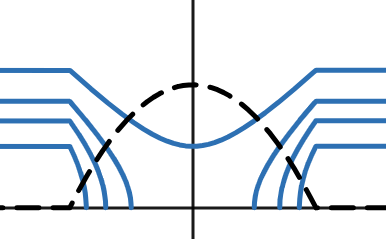
\includegraphics[width=0.3\textwidth]{classical-trajectories.png}
    \caption{Classical Phase space trajectories for the barrier potential $\varphi(x) = -\frac{1}{2}\omega^2x^2$} for the energies $0.25\varphi_{max}, 0.5\varphi_{max}, 0.75\varphi_{max},$ and $1.25\varphi_{max}$. The plot with $E = 1.25\varphi_{max}$ is the connected line.  The dotted line is $V(x)$.
    \label{fig:phase_space_barrier}
\end{figure}
Adding the imaginary time trajectory connecting the two parts, it will correspond to flipping the order of the terms in the square root in equation \ref{eq:classical-momentum}:
\begin{equation}
    \label{eq:imaginary-time-momentum}
    p = \pm 2m\sqrt{V(x) - E}
\end{equation}
giving the red plots in figure \ref{fig:phase_space_barrier_with_tunneling}.
\begin{figure}[h]
    \centering
    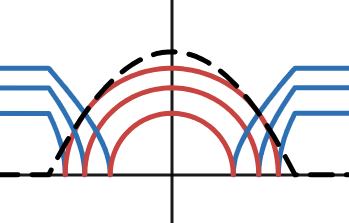
\includegraphics[width=0.3\textwidth]{classical-trajectories-with-tunneling.png}
    \caption{Classical Phase space trajectories for the barrier potential $\varphi(x) = -\frac{1}{2}\omega^2x^2$} for the energies $0.25\varphi_{max}, 0.5\varphi_{max},$ and $0.75\varphi_{max}$. The dotted line is $V(x)$. The red lines are the imaginary time trajectories connecting the two sides of the barrier.
    \label{fig:phase_space_barrier_with_tunneling}
\end{figure}
It is clear to see in figure \ref{fig:phase_space_barrier_with_tunneling} that the instanton trajectory connects to the two classical trajectories at $x = a$ and $x = b$, the points at whcih $E = V(x)$ on the two sides of the barrier, where the square roots in both equation \ref{eq:classical-momentum} and \ref{eq:imaginary-time-momentum} are zero. In this trajectories, the particle "moves" from one side and ends on the other side of the barrier.
\subsection{Energies above the barrier}
For an energy above the barrier, such as the top plot in \ref{fig:phase_space_barrier}
\end{document}